\subsection{Area 3 – Inserimento delle prenotazioni}
\begin{figure}[H]
\centering
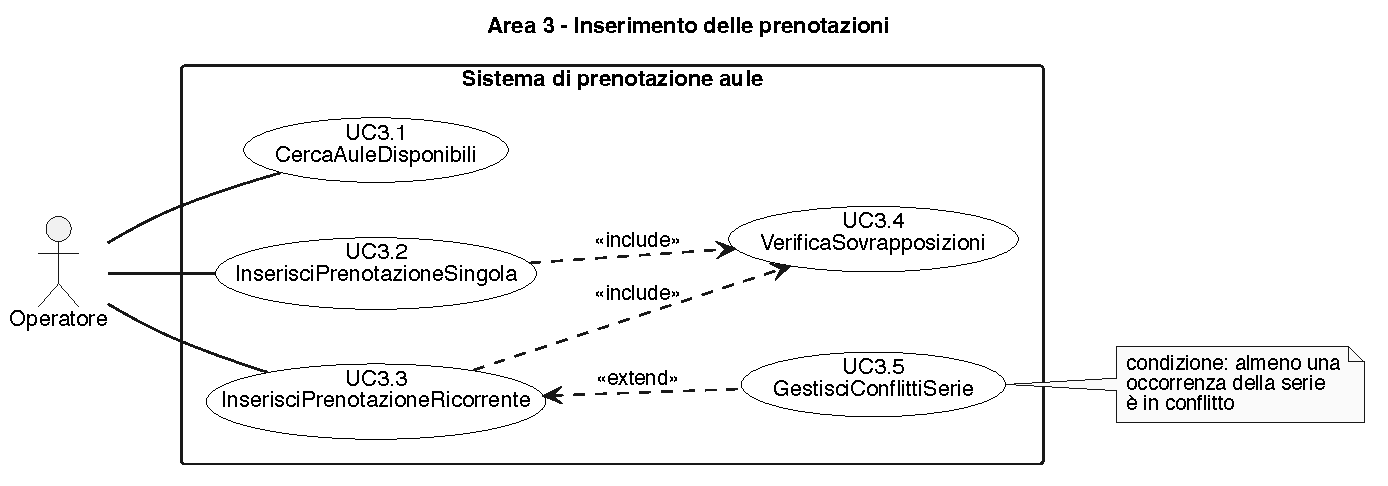
\includegraphics[width=\textwidth,height=0.8\textheight,keepaspectratio]{diagrammi/uc-area3-inserimento}
\caption{Casi d'uso dell'Area 3 – Inserimento delle prenotazioni}
\end{figure}

\subsubsection{[UC3.1] CercaAuleDisponibili}
\noindent Attore: Operatore\\
Requisiti correlati: FI3.1, FI3.7, ED3.4, ED3.5, ED3.8, IU3.2, IU4.6\\
Pre-condizioni: Nessuna oltre alla precondizione comune.\\
Post-condizioni: Il sistema mostra le aule senza prenotazioni sovrapposte alla fascia indicata. L'archivio è invariato.\\

\noindent Flusso principale:
\begin{enumerate}
\item L'Operatore apre la ricerca delle aule disponibili.
\item L'Operatore inserisce data, ora di inizio e ora di fine e avvia la ricerca.
\item Il sistema verifica che la fascia oraria sia valida (ED3.4, ED3.5).
\item Il sistema individua le aule che non hanno prenotazioni sovrapposte (ED3.8) alla fascia indicata.
\item Il sistema mostra le aule disponibili ordinate per codice, con codice, nome, edificio, piano e capienza.
\end{enumerate}
\noindent Flussi alternativi:
\begin{itemize}
\item \textbf{3a.} La fascia oraria non è valida (es. ora di fine non successiva all'ora di inizio, inizio nel passato):
\begin{itemize}
\item 3a.1 Il sistema indica il campo errato e il vincolo da rispettare;
\item 3a.2 si riprende dal passo 2.
\end{itemize}
\item \textbf{5a.} Nessuna aula è disponibile:
\begin{itemize}
\item 5a.1 Il sistema mostra il messaggio ``Nessuna aula disponibile nella fascia indicata''.
\end{itemize}
\item \textbf{5b.} L'Operatore seleziona un'aula tra i risultati e sceglie Prenota (FI3.7):
\begin{itemize}
\item 5b.1 Il sistema avvia UC3.2 InserisciPrenotazioneSingola con aula, data e fascia oraria già compilate.
\end{itemize}
\end{itemize}

\subsubsection{[UC3.2] InserisciPrenotazioneSingola}
\noindent Attore: Operatore\\
Requisiti correlati: FI3.2, FI3.4, FI3.5, ED3.1–ED3.5, ED3.8, IU3.1, IU4.6, IU4.7, NF7\\
Include: UC3.4 VerificaSovrapposizioni\\
Pre-condizioni: Nell'archivio sono registrati almeno un'aula e almeno un docente.\\
Post-condizioni: La prenotazione è registrata nell'archivio, l'archivio è salvato su file e la prenotazione compare nella lista delle prenotazioni.\\

\noindent Flusso principale:
\begin{enumerate}
\item L'Operatore sceglie il comando Nuova prenotazione.
\item Il sistema mostra il modulo di prenotazione (IU3.1) con l'opzione di ricorrenza disattivata.
\item L'Operatore sceglie aula, docente e tipo di attività, inserisce denominazione, data, ora di inizio e ora di fine e conferma.
\item Il sistema verifica che i dati rispettino i vincoli ED3.1–ED3.5.
\item Il sistema esegue UC3.4 VerificaSovrapposizioni sulla prenotazione.
\item Non ci sono conflitti: il sistema registra la prenotazione, salva l'archivio, chiude il modulo e mostra un messaggio di esito.
\end{enumerate}
\noindent Flussi alternativi:
\begin{itemize}
\item \textbf{1a.} Nell'archivio non ci sono aule o non ci sono docenti:
\begin{itemize}
\item 1a.1 Il sistema segnala che occorre prima registrare almeno un'aula e un docente e il caso d'uso termina.
\end{itemize}
\item \textbf{3a.} L'Operatore annulla: si applica FC1.
\item \textbf{3b.} L'Operatore attiva l'opzione di ricorrenza settimanale:
\begin{itemize}
\item 3b.1 il caso d'uso prosegue come UC3.3 InserisciPrenotazioneRicorrente dal passo 3.
\end{itemize}
\item \textbf{4a.} Uno o più dati non sono validi:
\begin{itemize}
\item 4a.1 Il sistema indica ogni campo errato e il vincolo da rispettare;
\item 4a.2 si riprende dal passo 3.
\end{itemize}
\item \textbf{6a.} UC3.4 ha trovato un conflitto:
\begin{itemize}
\item 6a.1 Il sistema mostra il motivo (aula occupata e/o docente impegnato) e i dati della prenotazione esistente in conflitto;
\item 6a.2 si riprende dal passo 3 con i dati già inseriti.
\end{itemize}
\item \textbf{6b.} Il salvataggio non riesce: si applica FC2.
\end{itemize}

\subsubsection{[UC3.3] InserisciPrenotazioneRicorrente}
\noindent Attore: Operatore\\
Requisiti correlati: FI3.3, FI3.4, FI3.5, ED3.1–ED3.8, IU3.1, IU4.6, IU4.7, NF7\\
Include: UC3.4 VerificaSovrapposizioni\\
Punto di estensione: Passo 7: almeno un'occorrenza è in conflitto $\rightarrow$ UC3.5 GestisciConflittiSerie.\\
Pre-condizioni: Nell'archivio sono registrati almeno un'aula e almeno un docente.\\
Post-condizioni: Tutte le occorrenze della serie sono registrate nell'archivio con lo stesso identificativo di serie, l'archivio è salvato su file e le occorrenze compaiono nella lista delle prenotazioni.\\

\noindent Flusso principale:
\begin{enumerate}
\item L'Operatore sceglie il comando Nuova prenotazione.
\item Il sistema mostra il modulo di prenotazione (IU3.1).
\item L'Operatore sceglie aula, docente e tipo di attività, inserisce denominazione, data della prima occorrenza, ora di inizio e ora di fine, attiva la ricorrenza settimanale, inserisce la data di termine e conferma.
\item Il sistema verifica che i dati rispettino i vincoli ED3.1–ED3.6.
\item Il sistema calcola le date delle occorrenze: dalla data della prima occorrenza, ogni 7 giorni, fino alla data di termine inclusa (ED3.6).
\item Il sistema esegue UC3.4 VerificaSovrapposizioni su tutte le occorrenze.
\item Nessuna occorrenza è in conflitto: il sistema registra tutte le occorrenze con un nuovo identificativo di serie (ED3.7), salva l'archivio, chiude il modulo e mostra un messaggio con il numero di occorrenze create.
\end{enumerate}
\noindent Flussi alternativi:
\begin{itemize}
\item \textbf{1a.} Nell'archivio non ci sono aule o non ci sono docenti:
\begin{itemize}
\item 1a.1 Il sistema segnala che occorre prima registrare almeno un'aula e un docente e il caso d'uso termina.
\end{itemize}
\item \textbf{3a.} L'Operatore annulla: si applica FC1.
\item \textbf{3b.} L'Operatore disattiva l'opzione di ricorrenza:
\begin{itemize}
\item 3b.1 il caso d'uso prosegue come UC3.2 InserisciPrenotazioneSingola dal passo 3.
\end{itemize}
\item \textbf{4a.} Uno o più dati non sono validi (compresa una data di termine a meno di 7 giorni dalla prima occorrenza):
\begin{itemize}
\item 4a.1 Il sistema indica ogni campo errato e il vincolo da rispettare;
\item 4a.2 si riprende dal passo 3.
\end{itemize}
\item \textbf{7a.} UC3.4 ha trovato conflitti per almeno un'occorrenza:
\begin{itemize}
\item 7a.1 si esegue UC3.5 GestisciConflittiSerie.
\end{itemize}
\item \textbf{7b.} Il salvataggio non riesce: si applica FC2.
\end{itemize}

\subsubsection{[UC3.4] VerificaSovrapposizioni}
\noindent Attore: — (caso d'uso incluso da UC3.2 e UC3.3; non è avviato direttamente dall'Operatore)\\
Requisiti correlati: FI3.4, FI3.5, ED3.8, NF7\\
Pre-condizioni: Sono disponibili i dati validi di una o più prenotazioni da inserire (aula, docente, data, ora di inizio, ora di fine).\\
Post-condizioni: È disponibile l'elenco dei conflitti trovati (vuoto se non ce ne sono); per ogni conflitto: data, motivo e prenotazione esistente coinvolta. L'archivio è invariato.\\

\noindent Flusso principale:
\begin{enumerate}
\item Per ogni prenotazione da inserire, il sistema cerca nell'archivio le prenotazioni della stessa data la cui fascia oraria si sovrappone (ED3.8).
\item Per ciascuna prenotazione sovrapposta, se riguarda la stessa aula il sistema registra un conflitto con motivo ``aula occupata'' (FI3.4).
\item Per ciascuna prenotazione sovrapposta, se riguarda lo stesso docente il sistema registra un conflitto con motivo ``docente impegnato'' (FI3.5).
\item Il sistema restituisce l'elenco dei conflitti al caso d'uso che lo ha incluso.
\end{enumerate}
\noindent Flussi alternativi:
\begin{itemize}
\item \textbf{2a.} Una prenotazione sovrapposta riguarda sia la stessa aula sia lo stesso docente:
\begin{itemize}
\item 2a.1 il conflitto viene registrato con entrambi i motivi.
\end{itemize}
\end{itemize}

\subsubsection{[UC3.5] GestisciConflittiSerie}
\noindent Attore: Operatore\\
Requisiti correlati: FI3.6, IU3.3, IU4.7, ED3.7, NF7\\
Estende: UC3.3 InserisciPrenotazioneRicorrente, quando almeno un'occorrenza della serie è in conflitto.\\
Pre-condizioni: UC3.4 ha trovato conflitti per almeno un'occorrenza della serie che l'Operatore sta inserendo.\\
Post-condizioni: Se l'Operatore sceglie di salvare le date libere: le sole occorrenze senza conflitti sono registrate con lo stesso identificativo di serie e l'archivio è salvato su file. Negli altri casi l'archivio è invariato.\\

\noindent Flusso principale:
\begin{enumerate}
\item Il sistema mostra la finestra dei conflitti (IU3.3): numero di occorrenze in conflitto sul totale e, per ogni occorrenza in conflitto, data, motivo e prenotazione esistente.
\item Il sistema propone le scelte ``Salva solo le date libere'', ``Modifica dati'' e ``Annulla''.
\item L'Operatore sceglie ``Salva solo le date libere''.
\item Il sistema registra le occorrenze senza conflitti con un nuovo identificativo di serie, salva l'archivio, chiude il modulo e mostra un messaggio con il numero di occorrenze create e le date saltate.
\end{enumerate}
\noindent Flussi alternativi:
\begin{itemize}
\item \textbf{2a.} Tutte le occorrenze sono in conflitto:
\begin{itemize}
\item 2a.1 Il sistema propone solo ``Modifica dati'' e ``Annulla'';
\item 2a.2 si prosegue dal passo 3 con una di queste due scelte.
\end{itemize}
\item \textbf{3a.} L'Operatore sceglie ``Modifica dati'':
\begin{itemize}
\item 3a.1 Il sistema chiude la finestra dei conflitti e torna al modulo di prenotazione con i dati già inseriti;
\item 3a.2 si riprende dal passo 3 di UC3.3.
\end{itemize}
\item \textbf{3b.} L'Operatore sceglie ``Annulla'': si applica FC1.
\item \textbf{4a.} Il salvataggio non riesce: si applica FC2.
\end{itemize}
